\section{Background}
\label{sec:lts-transformation:background}
In this section, we introduce the basic concepts required to introduce our preservation check.
First, finite state LTSs are introduced, which we use to define the behavior of individual processes as well as the behavior of models formed by interacting processes.
Then, we discuss networks of LTSs, which are used to specify models in terms of interacting processes.
Next, we give a definition of DSBB, an equivalence relation between LTSs.
Finally, a fragment of the modal $\mu$-calculus~\cite{Kozen-83} that is compatible with DSBB is discussed.





\subsection{Labeled transition system}
An LTS~\graph is a tuple~\ltstuple{\graph}, where \states{\graph} is the (finite) set of states, $\actions{\graph}$ is the set of actions (including the invisible action $\tau$), $\transitions{\graph} \subseteq \states{\graph} \times \actions{\graph} \times \states{\graph}$ is the transition relation, and $\initialstates{\graph} \subseteq \states{\graph}$ the set of initial states.
Usually, LTSs representing potential behavior of concurrent systems have only one initial state, as defined in Section~\ref{sec:reusable-correct-transformations:operational_semantics}.
Here, we support multiple initial states to enable representing transformation rule patterns in terms of LTSs, as described in Section~\ref{sec:lts-transformation:transformations}.
In all other cases, LTSs have a single initial state.
Actions in \actions{\graph} are denoted by $a$, $b$, $c$, etc.
We use $s_1 \xrightarrow{a}_\graph s_2$ as a shorthand for $\langle s_1, a, s_2 \rangle \in \transitions{\graph}$.
If a transition $s_1 \xrightarrow{a}_\graph s_2$ is an element of $\transitions{\graph}$, this means that the LTS~\graph can move from state~$s_1$ to state~$s_2$ by performing action $a$.
The reflexive transitive closure of $\xrightarrow{\tau}_\graph$ is denoted by $\tausteps_\graph$.







\subsection{Network of LTSs}
We represent models consisting of a finite number of concurrent processes by a number of LTSs and a set of rules that define how these LTSs interact.
For this, we use the concept of networks of LTSs~\cite{lang05}.
Given an integer $n>0$, $1..n$ is the set of integers ranging from $1$ to $n$.
A vector $\vectornot{v}$ of size $n$ contains $n$ elements indexed by $1..n$. For $i \in 1..n$, $\vectornot{v}[i]$ denotes element $i$ in $\vectornot{v}$.
	
\begin{definition}
A network of LTSs~\smodel of size~$n$ is a pair~\networktuple, where
\begin{itemize}
\item $\Pi$ is vector of $n$ ({\it process}) LTSs.
For each $i \in 1..n$, we write $\Pi[i] = \ltstuple{i}$, and $s_1\xrightarrow{b}_i s_2$ is shorthand for $s_1\xrightarrow{b}_{\Pi[i]} s_2$;
\item \synchrules is a finite set of synchronization rules.
A synchronization rule is a tuple \syncruletuple, where $a$ is an action label, and $\vectornot{t}$ is a vector of size $n$ called a synchronization vector, whose elements are action labels from $\bigcup_{i\in 1..n} \actions{i}$ and a special symbol $\bullet$ that does not occur as a label in the LTSs.
If~$\vectornot{t}[i] = \bullet$ for some synchronization rule, then process LTS~$i$ is not involved in this synchronization.
\end{itemize}
\end{definition}

The potential behavior of a network of LTSs can be described as a single LTS.
For a network~$\smodel = \networktuple$, combining the LTSs in $\Pi$ according to the rules in $\synchrules$ produces a new LTS~\ltstuple{\smodel}, where
\begin{itemize}
\item $\initialstates{\smodel} = \{ \langle s_{1},\ldots, s_{n} \rangle \mid \forall i \in 1..n . s_{i} \in \initialstates{i} \}$;
\item $\actions{\smodel} = \{a \mid \langle \vectornot{t}, a \rangle \in \synchrules \}$;
\item $\states{\smodel} = \states{1} \times \ldots \times \states{n}$;
\item $\transitions{\smodel}$ is the smallest transition relation satisfying:
\[
\langle \vectornot{t}, a \rangle \in \synchrules \wedge \forall i \in 1..n . (\vectornot{t}[i] = \bullet \wedge s'[i]=s[i]) \vee (\vectornot{t}[i] \neq \bullet \wedge s[i]\xrightarrow{\vectornot{t}[i]}_i s'[i]) \implies s\xrightarrow{a}_{\smodel} s'.
\]
\end{itemize}

\noindent
In the remainder, we refer to such an LTS as a network LTS.

%%%%%%%%%%%%%%%%%%%%%%%%%%%%%%%%%%%%%%%%%%%%%%%%%%%%%%%%%
%%%%%%%%%%%%%%%%%%%%%%%%%%%%%%%%%%%%%%%%%%%%%%%%%%%%%%%%%
%%%%%%%%%%%%%%%%%%%%%%%%%%%%%%%%%%%%%%%%%%%%%%%%%%%%%%%%%
%%%With $\vectornot{s}\xrightarrow{b}_\smodel^{\vectornot{t}} \vectornot{s}'$, we denote that $\vectornot{t}$ enables $\vectornot{s}\xrightarrow{b}_\smodel \vectornot{s}'$.
%%%%%%%%%%%%%%%%%%%%%%%%%%%%%%%%%%%%%%%%%%%%%%%%%%%%%%%%%
%%%%%%%%%%%%%%%%%%%%%%%%%%%%%%%%%%%%%%%%%%%%%%%%%%%%%%%%%
%%%%%%%%%%%%%%%%%%%%%%%%%%%%%%%%%%%%%%%%%%%%%%%%%%%%%%%%%

\begin{figure}[hbt]
\centering
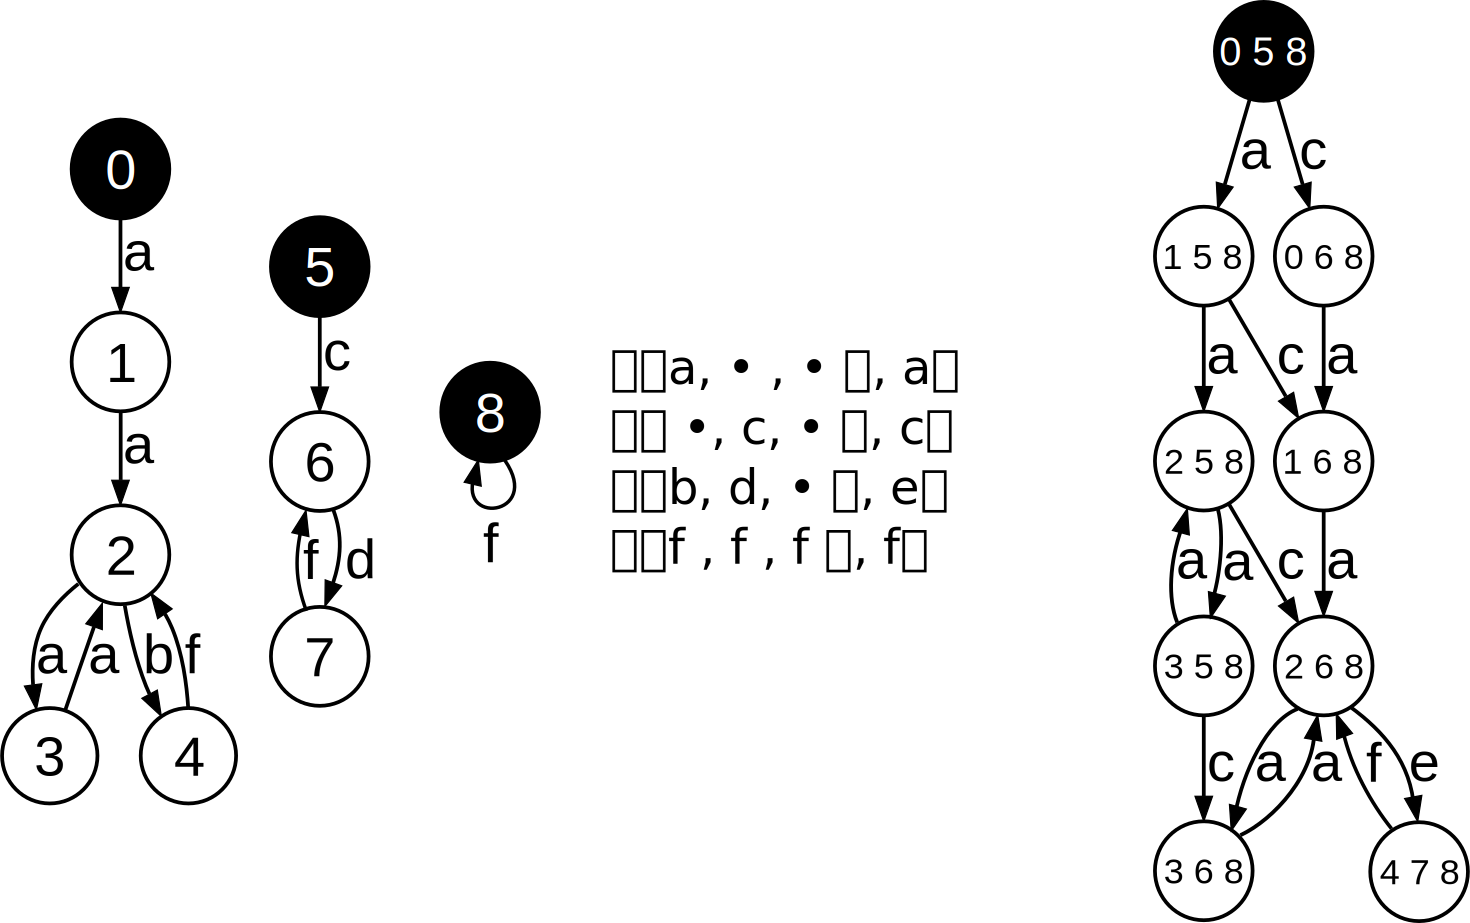
\includegraphics[scale=0.2]{lts-transformation/figs/network}
\caption{A network of LTSs and the corresponding network LTS}
\label{fig:lts-transformation:network}
\end{figure}

On the left of Figure~\ref{fig:lts-transformation:network}, a network consisting of three process LTSs and four synchronization rules is shown.
The network LTS representing the behavior of this network is shown on the right of the figure.
The figure demonstrates the expressiveness of networks of LTSs.
It shows, for example, that multi-party synchronization is offered, as illustrated with the synchronization rule~$\langle\langle f, f, f\rangle, f\rangle$.
This rule specifies that the action~$f$ in the network LTS is the result of the synchronization of the actions~$f$ of the three processes.
Rule~$\langle\langle b, d, \bullet \rangle, e\rangle$ specifies a synchronization between processes~$\Pi[1]$ and~$\Pi[2]$, rule~$\langle\langle a, \bullet, \bullet \rangle, a \rangle$ specifies that action~$a$ of process~$\Pi[1]$ can be executed independently, and rule~$\langle\langle \bullet, c, \bullet \rangle, c \rangle$ specifies the same for action~$c$ of process~$\Pi[2]$.
Synchronization rules can also be used to introduce non-deterministic behavior, by specifying multiple rules involving the same actions.
For example, by adding the rule~$\langle\langle a, c, \bullet \rangle, g \rangle$ to the network of Figure~\ref{fig:lts-transformation:network}, $\Pi[1]$ and~$\Pi[2]$ can either synchronize or perform action~$a$ and~$c$ independently.

To abstract from certain actions, we define the hiding operator $\abstr$, which renames all actions in~$H$ to~$\tau$.
This operator can be extended to networks of LTSs.

\begin{definition}
\label{def:lts-transformations:hiding}
Let \actions{} be a set of actions and $H \subseteq \actions{}$.
The hiding of an action $a \in \actions{}$ w.r.t.\ $H$ is defined as follows.
\[
\abstr (a) =
\left\{\begin{array}{ll}
a    & {\rm if} ~ a \not\in H \\
\tau & {\rm if} ~ a \in H
\end{array}\right.
\]
The hiding of a network $\smodel = \langle \Pi, \synchrules \rangle$ w.r.t.\ $H$ is defined as follows.
\[
	\abstr (\langle \Pi, \synchrules \rangle) =
	\langle
		\Pi,
		\{\langle \vectornot{t}, \abstr(a)\rangle \mid \langle \vectornot{t}, a \rangle \in \synchrules \}
	\rangle
\]
\end{definition}





\subsection{Divergence-Sensitive Branching Bisimilarity}
We use the equivalence relation DSBB~\cite{GlaLutTrc09} to relate LTSs, which preserves $\tau$-cycles and branching-time properties such as inevitable reachability.

\begin{definition}
\label{def:lts-transformation:dsbbsim}
For LTSs $\graph_1 = \ltstuple{\graph_1}$ and~$\graph_2 = \ltstuple{\graph_2}$, a binary relation $B \subseteq \states{\graph_1} \times \states{\graph_2} $ is a divergence-sensitive branching bisimulation if for all $s \in \states{\graph_1}$ and $t \in \states{\graph_2}$ such that $s\ B\ t$, the following conditions hold.
\begin{enumerate}
\item If $s \xrightarrow{a}_{\graph_1} s'$ then
  \begin{itemize}
  \item either $a=\tau$ with $s'\ B\ t$;
  \item or $t \tausteps_{\graph_2} {\hat t} \xrightarrow{a}_{\graph_2} t'$ with $s\ B\ {\hat t}$ and $s'\ B\ t'$.
  \end{itemize}
\item Symmetrically, if $t \xrightarrow{a}_{\graph_2} t'$ then
  \begin{itemize}
  \item either $a=\tau$ with $s\ B\ t'$;
  \item or $s \tausteps_{\graph_1} {\hat s} \xrightarrow{a}_{\graph_1} s'$ with ${\hat s}\ B\ t$ and $s'\ B\ t'$.
  \end{itemize}
\item If for all $k\geq 0$ and $s=s_0$, $s_k \xrightarrow{\tau}_{\graph_1} s_{k+1}$ then for all $\ell\geq 0$ and $t=t_0$, $t_\ell \xrightarrow{\tau}_{\graph_2} t_{\ell+1}$ and $s_k\ B\ t_{\ell}$, for all $k, \ell$.
\item Symmetrically, if for all $k\geq 0$ and $t=t_0$, $t_k \xrightarrow{\tau}_{\graph_2} t_{k+1}$ then for all $\ell\geq 0$ and $s=s_0$, $s_\ell \xrightarrow{\tau}_{\graph_1} s_{\ell+1}$ and $s_{\ell}\ B\ t_k$, for all $k, \ell$.
\end{enumerate}
Two states $s$ and $t$ are divergence-sensitive branching bisimilar, denoted by $s\dsbbis t$, if there is a divergence-sensitive branching bisimulation~$B$ with $s\ B\ t$.
\end{definition}

Two LTSs~$\graph_1 = \ltstuple{\graph_1}$ and~$\graph_2 = \ltstuple{\graph_2}$ are divergence-sensitive branching bisimilar, denoted by $\graph_1 \dsbbis \graph_2$, iff $\forall s_1 \in \initialstates{\graph_1}. \exists s_2 \in \initialstates{\graph_2}. s_1 \dsbbis s_2$ and vice versa.
Furthermore, a state $s$ is diverging, denoted by $s\diverge$, iff an infinite $\tau$-path is reachable from~$s$.
For finite LTSs, this means that a $\tau$-cycle is reachable via $\tau$-transitions.

If the constituting LTSs satisfy the following conditions related to $\tau$-transitions, DSBB is a congruence for networks of LTSs,
which means that replacing a process LTS in a network with a process LTS that is divergence-sensitive branching bisimilar leads to a network for which the corresponding network LTS is divergence-sensitive branching bisimilar with the network LTS that corresponds to the original network.

\begin{definition}
\label{def:lts-transformation:admissibility}
A network $\smodel = \networktuple$ is called admissible iff the following holds.
\begin{enumerate}
\item \textbf{No synchronization and renaming:}
\[
\forall \syncruletuple \in \synchrules. \vectornot{t}[i] = \tau \implies {\it Ac}(\vectornot{t}) = \{i\} \wedge a=\tau;
\]
\item \textbf{No cut:} $\exists s_1, s_2 \in \states{i}. s_1\xrightarrow{\tau}_i s_2 \implies \exists \langle \vectornot{t}, \tau \rangle \in \synchrules. \vectornot{t}[i] = \tau$,
\end{enumerate}
\end{definition}

\noindent
where the set~${\it Ac}(\vectornot{t})$ of indices of processes active for a synchronization vector~$\vectornot{t}$ is defined as ${\it Ac}(\vectornot{t})= \{i \mid i \in 1..n \wedge \vectornot{t}[i] \neq \bullet \}$.
The first condition states that a $\tau$-action may not synchronize with other actions and that it may not be renamed, and the second condition states that there must exist synchronization rules that enable the $\tau$-transitions of each process.
In the remainder of this chapter, only admissible networks are considered.

\subsection{The modal $\mu$-calculus \dsbrLmu}
\label{subsec:lts-transformation:lmu}
Mateescu and Wijs~\cite{mateescu.wijs.propred} identified a fragment of the modal $\mu$-calculus~\cite{Kozen-83} that is fully compatible with the maximal hiding technique~\cite{mateescu.wijs.propred} and DSBB.
The fragment is called~\dsbrLmu and is suitable for expressing safety, liveness, and fairness properties.
In~\dsbrLmu, properties are expressed in terms of action formulas, denoted by $\Af$, and state formulas, denoted by $\Sf$ and $\Sp$.
The syntax of these formulas and the semantics of the action formulas are defined as follows.

\[
\begin{array}{lcl}
\Af & {::=} & a \mid \FALSE \mid \neg \Af_1 \mid \Af_1 \vee \Af_2
\end{array}
\]

\[
\begin{array}{rcl}
\sem a \antic_{\actions{}} & = & \{ a \} \\
\sem \FALSE \antic_{\actions{}} & = & \emptyset \\
\sem \neg \Af_1 \antic_{\actions{}} & = & {\actions{}} \setminus \sem \Af_1 \antic_{\actions{}} \\
\sem \Af_1 \vee \Af_2 \antic_{\actions{}} & = & \sem \Af_1 \antic_{\actions{}} \cup \sem \Af_2 \antic_{\actions{}}
\end{array}
\]

\[
\begin{array}{rcl}
\Sf & {::=} & \FALSE
 \mid \neg \Sf_1
 \mid \Sf_1 \vee \Sf_2
 \mid \langle (\Sf_1 ? . \Af_h)^{*} \rangle \Sp
 \mid \langle \Sf_1 ? . \Af_h \rangle @
 \mid X
 \mid \mu X . \Sf_1 \\
\Sp & {::=} & \Sf
 \mid \langle \Af_v \rangle \Sf
 \mid \neg \Sp_1
 \mid \Sp_1 \vee \Sp_2,
\end{array}
\]

\noindent
where $\actions{}$ is a set of actions, $X$ is a set of propositional variables, $\tau \in \sem \Af_h \antic_{\actions{}}$, and~$\tau \not\in \sem \Af_v \antic_{\actions{}}$.

Interpretation $\sem \Af \antic_\actions{}$ of $\Af$ on the set of actions $\actions{}$ denotes the set of actions satisfying~$\Af$.
An action $a$ satisfies a formula $\Af$, denoted by $a \models_\actions{} \Af$, iff $a \in \sem \Af \antic_\actions{}$.
Furthermore, a transition~$s_1\ \smash{\xrightarrow{a}_\graph}\ s_2$ with~$a \models_\actions{\graph} \Af$ is called an $\Af$-transition.

We do not provide the formal semantics of the state formulas, as it is not essential for understanding the current work.
Compared to the standard modal $\mu$-calculus, the fragment~\dsbrLmu differs in two respects.
First, it introduces the weak possibility modality and the weak infinite looping operator.
Informally, the weak possibility modality~$\langle (\Sf_1 ? . \Af_h)^{*} \rangle \Sp$ characterizes the states having an outgoing sequence of zero or more $\Af_h$-transitions whose intermediate states satisfy~$\Sf_1$ and whose terminal state satisfies~$\Sp$.
The weak infinite looping operator~$\langle \Sf_1 ? . \Af_h \rangle @$ characterizes the states having an infinite outgoing sequence of~$\Af_h$-transitions whose intermediate states satisfy~$\Sf_1$.
In both cases, $\Af_h$ must capture~$\tau$.
Second, the occurrence of the strong modality~$\langle \Af_v \rangle \Sf$ is restricted syntactically such that it can appear only after a weak possibility modality, and the action formula~$\Af_v$ must denote visible actions only.
For further details, we refer to the work of Mateescu and~Wijs~\cite{mateescu.wijs.propred}.

The fact that a state~$s$ of an LTS~\graph satisfies a closed state formula~$\Sf$ is denoted by~$s \models_\graph \Sf$.
A formula is closed if all propositional variables are bound.
Additionally, we denote~$\forall s \in \initialstates{\graph} . s \models_\graph \Sf$ by~$\models_\graph \Sf$.

When checking a state formula $\Sf$ on an LTS, some actions can be hidden (renamed to~$\tau$) without disturbing the interpretation of~$\Sf$.

\begin{definition}
\label{def:lts-transformation:hiding-set}
Let $\Af$ be an action formula interpreted over a set of actions $\actions{}$.
The hiding set of $\Af$ w.r.t.\ $\actions{}$ is defined as follows.
\[
h_\actions{} (\Af) = \left\{
\begin{array}{ll}
\sem \Af \antic_\actions{}                    & {\rm if} ~ \tau \models \Af \\
\actions{} \setminus \sem \Af \antic_\actions{} & {\rm if} ~ \tau \not\models \Af
\end{array}
\right.
\]
The hiding set of a state formula $\Sf$ w.r.t.\ $\actions{}$, denoted by $h_\actions{} (\Sf$), is defined as the intersection of $h_\actions{} (\Af)$ for all action subformulas $\Af$ of $\Sf$.
\end{definition}

We denote maximal hiding in an LTS~$\graph = \ltstuple{\graph}$ as $\maxabstr(\graph) = \smash{\abstrset{h_{\actions{\graph}}(\Sf)}(\graph)}$.
Maximal hiding preserves~\dsbrLmu properties: $\models_\graph \Sf \iff \smash{\models_{\maxabstr(\graph)} \Sf}$.
Furthermore, for closed $\Sf$, \dsbrLmu is compatible with the $\dsbbis$ relation.
Let $\graph = \ltstuple{\graph}$ be an LTS and let $s_1, s_2 \in \states{\graph}$ such that $s_1 \dsbbis s_2$.
Then, $s_1 \models_\graph \Sf \iff s_2 \models_\graph \Sf$ for any closed state formula $\Sf$ of \dsbrLmu.
This allows reducing an LTS (after maximal hiding) modulo DSBB before verifying a closed~\dsbrLmu formula~\cite{mateescu.wijs.propred}.
It also allows reasoning about LTSs w.r.t.\ properties.
Given a~\dsbrLmu formula $\Sf$ and LTSs~$\graph_1$ and $\graph_2$ with $\maxabstr(\graph_1) \dsbbis \maxabstr(\graph_2)$, then, if~$\models_{\graph_1} \Sf$, also $\models_{\graph_2} \Sf$. 